\documentclass{whswinvcbook}
\usepackage{whswinvcgsp}

\usepackage[ngerman]{babel} % language selection: english/ngerman
                            % note: delete all output files on language change
\usepackage[utf8]{inputenc} % allow for using umlauts
\usepackage{lipsum}         % provide lorem ipsum ...
\usepackage{siunitx}        % provide SI units
\usepackage{amsfonts}       % Provides hollow R for real numbers, hollow C for complex numbers, etc.
\usepackage{algorithm}      % Provides Border for Pseudocode
\usepackage{algpseudocode}  % Provides Pseudocode
\usepackage{interval}       % Provides proper intervals
\usepackage{listings}       % Provides Source Code Listing
\usepackage{gensymb}        % Provides the degree symbol
\usepackage{wrapfig}        % Provides wrapping of text around figures
\usepackage{amssymb}        % Provides empty set symbol (\varnothing)
\usepackage{colortbl}
\usepackage{varwidth}

\title[Bericht]{Classcon Consulting GmbH}
\subtitle{d.velop AG}
\author[Nico Pistel]{Nico Pistel}
\summerterm{2019}

\definecolor{bluekeywords}{rgb}{0,0,1}
\definecolor{greencomments}{rgb}{0,0.5,0}
\definecolor{redstrings}{rgb}{0.64,0.08,0.08}
\definecolor{xmlcomments}{rgb}{0.5,0.5,0.5}
\definecolor{types}{rgb}{0.17,0.57,0.68}

\lstset{language=[Sharp]C,
captionpos=b,
%numbers=left, %Nummerierung
%numberstyle=\tiny, % kleine Zeilennummern
frame=lines, % Oberhalb und unterhalb des Listings ist eine Linie
showspaces=false,
showtabs=false,
breaklines=true,
showstringspaces=false,
breakatwhitespace=true,
escapeinside={(*@}{@*)},
commentstyle=\color{greencomments},
morekeywords={partial, var, value, get, set},
keywordstyle=\color{bluekeywords},
stringstyle=\color{redstrings},
basicstyle=\ttfamily\small,
}

\makeatletter
\newcommand{\thickhline}{%
    \noalign {\ifnum 0=`}\fi \hrule height 1pt
    \futurelet \reserved@a \@xhline
}
\newcolumntype{T}{@{\hskip\tabcolsep\vrule width 1pt\hskip\tabcolsep}}
\makeatother

\usepackage{scrlayer-scrpage}
\clearpairofpagestyles
\chead{\headmark}
\cfoot*{\pagemark}

\begin{document}

\frontmatter

\maketitle

\cleardoublepage
\chapter*{Abstract}
Im Rahmen der Praxisphase wurde ein 12-wöchiges Praktikum bei der Classcon Consulting GmbH absolviert. Da sich das Unternehmen hauptsächlich mit Dokumentklassifizierung beschäftigt, sind die in diesem Bericht beschriebenen Aufgaben auch in diesem Bereich angesiedelt. Dabei wurde sich zunächst mit AWS Textract - einem neuen OCR Dienst von Amazon - beschäftigt. Als Ergebnis wurde ein Cloud-Dienst entwickelt, welcher Dokumente asynchron mit Textract auswertet und das Ergebnis in eine betriebsinterne XML-Struktur schreibt, welche zur weiteren Klassifizierung von anderen Diensten wieder herangezogen wird. Der Dienst wurde ausführlich getestet und die Ergebnisse, welche der Dienst mit bestimmten Beispieldokumenten liefert, protokolliert. Nach Abschluss der ersten Aufgabe wurde sich noch mit der statistischen Auswertung der Attributsextraktion der Klassifizierungssoftware beschäftigt, womit auch die Ergebnisse des Dienstes ausgewertet wurden und damit die Erkennungsqualität bewertet werden kann.

\tableofs
\lstlistoflistings

\mainmatter

\chapter{Einführung}
\section{Betriebsbeschreibung}
Die Classcon Consulting GmbH ist ein Tochterunternehmen der d.velop AG. Dabei fokussiert sich die Classcon Consulting GmbH auf die teil- und vollautomatische Erschließung von Dokumenten. Dabei wird auf verschiedenste Ansätze aus dem Bereich der maschinellen Klassifizierung und Datenextraktion aufgesetzt. Des Weiteren hilft die Classcon Consulting GmbH dabei, Geschäftsprozesse zu automatisieren, um die Wettbewerbsposition der Kunden zu verbessern.
\section{Software}
Die Lösungen der Classcon Consulting GmbH umfassen das Capturing und das automatische Klassifizieren und Extrahieren von Daten aus Dokumenten. Diese Lösungen sind hauptsächlich auf zwei Softwarepakete aufgeteilt: d.capture batch und das Hauptprodukt der Classcon Consulting GmbH - d.classify.
\subsection{d.capture batch}
Die d.capture batch stellt das Hauptprodukt der d.velop AG dar und ist ein Softwarepaket, welches die Funktionalität einer Scan-Software durch weitere Funktionalitäten ergänzt. Dazu gehört die Texterkennung durch eine OCR-Engine, die Validierung der erkannten Daten mit Abgleich an eine Datenbank und das Exportieren der Daten in gängige Warenwirtschaftssysteme. Die d.capture batch arbeitet stapelorientiert. Ein Stapel gehört einer Stapelklasse an, welche beschreibt, wie die Dokumente eines Stapels verarbeitet werden sollen. Bei der Verarbeitung werden mehrere Positionen (wie z.\,B. Texterkennung oder Validierung) für jedes Dokument im Stapel sequenziell abgearbeitet. Es können auch eigene Positionen von Hand programmiert werden, wozu die d.capture batch eine API bereitstellt, die in VBScript ansprechbar ist.
\begin{figure}[H]
    \centering
    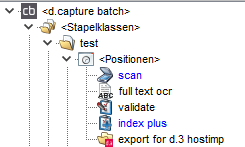
\includegraphics[width=0.60\textwidth]{img/dcapture_positionen.png}
    \caption{Eine Stapelklasse in d.capture batch mit 5 Positionen}
    \label{fig-dcapture-positionen}
\end{figure}
\subsection{d.classify}
Die Klassifizierungssoftware, welche von d.capture batch verwendet wird, stellt mit d.classify das Hauptprodukt der Classcon Consulting GmbH dar. Die Klassifizierung per d.classify kann als Position einer Stapelklasse in d.capture batch eingebunden werden. Die Software lässt sich aber auch unabhängig von anderen d.velop Produkten verwenden.

Die Klassifizierung in d.classify läuft entweder rein textbasiert ab oder mit grafischer Unterstützung. Bei einer reinen textbasierten Klassifizierung wird anhand des per OCR erkannten Textes probiert, Attribute (wie z.\,B. Rechnungsnummer oder Rechnungsdatum) herauszufiltern. Dazu werden Ausprägungen dieser Attribute angelegt, welche definieren, wann ein Teil des Textes als ein bestimmtes Attribut gilt. Diese Ausprägungen werden entweder als reguläre Ausdrücke formuliert (was sich z.\,B. gut dazu eignet, um ein Datum oder eine E-Mail-Adresse auf einem Dokument zu erkennen) oder als Stringvergleich mit einer gegebenen Maximalabweichung von einem Referenzstring (Fuzzy-String-Matching). Um die Suche nach Attributen zu verbessern, werden bei der grafisch unterstützten Suche nur die Teile des Textes durchsucht, die sich in einem bestimmten grafischen Bereich des Dokumentes befinden. Dieser Bereich wird entweder absolut zur Seite von Hand angegeben (so könnte man z.\,B. für das Attribut Seitenzahl jede Ecke und Kante des Dokumentes als eine solche Ausprägung anlegen) oder bezieht sich relativ auf einen bestimmten Teil des Dokumentes. Dieser Teil wird als Anker bezeichnet und kann abermals nach den gleichen Verfahren im Dokument gefunden werden. Somit lässt sich z.\,B. zunächst das Wort Telefonnummer auf dem Dokument suchen, dieses wird dann als Anker für die eigentliche Ausprägung (die Nummer) verwendet, dafür wird ein Suchbereich relativ zum Anker angegeben (z.\,B. rechts vom Wort).

Im unteren Beispiel ist zu sehen, wie eine Rechnungsnummer von einem Dokument extrahiert wird. Zunächst wird das Wort Rechnungsnummer als Ankerbegriff festgelegt. Dieser Begriff wird in dem roten Bereich auf dem Dokument gesucht (der rote Bereich war hier die obere Hälfte des Dokumentes). Der Begriff wurde gefunden und grün markiert. Zur eigentlichen Extraktion wird nun mithilfe des gefundenen Ankerbegriffes ein neuer Bereich (blau markiert) unterhalb des Ankers definiert. In diesem Begriff wird die eigentliche Rechnungsnummer gesucht. Dazu wird in diesem Bereich lediglich mit einem regulären Ausdruck nach einer Zeichenfolge gesucht, die nur aus den Ziffern 0-9 besteht.
\begin{figure}[H]
    \centering
    \subfloat[Festlegung des Ankerbegriffes\label{fig-classify-anker}]{
      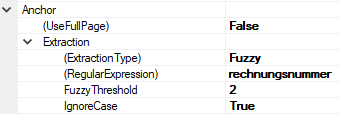
\includegraphics[width=0.48\linewidth]{img/dclassify_anker.png}
    }
    \hfill
    \subfloat[Extraktionseinstellungen\label{fig-classify-extraktion}]{
      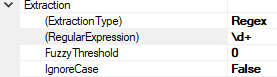
\includegraphics[width=0.48\linewidth]{img/dclassify_extraktion.png}
    }
    \hfill
    \subfloat[Erkennung im Dokument\label{fig-dclassify-rechnungsnummer}]{
      
\includegraphics[width=1.0\linewidth]{img/dclassify_rechnungsnummer.png}
    }
    \caption{Extraktion einer Rechnungsnummer in d.classify}
    \label{fig-dclassify}
\end{figure}
\chapter{Amazon Textract}
\section{Motivation}
Bevor ein Dokument klassifiziert werden kann, muss zunächst der Text des Dokumentes extrahiert werden. Diese Texterkennung (OCR vom englischen Optical Character Recognition) wird von einer separaten OCR-Engine übernommen. Normalerweise müssten Kunden, die ihre Dokumente automatisiert klassifizieren lassen möchten, somit eine Lizenz für eine von d.capture unterstützte OCR-Engine kaufen, um das volle Softwarepaket verwenden zu können. Außerdem muss die Engine lokal beim Kunden installiert werden, was weiteren Aufwand verursacht und mehr Rechenleistung beim Kunden voraussetzt. Die beiden aktuell unterstützten OCR-Engines sind ABBYY FineReader und Tesseract OCR von Google.

Eine mögliche neue Alternative ist, dass die Texterkennung nicht lokal beim Kunden durchgeführt wird, sondern zentral auf einem d.velop-Server. Dazu werden die Dokumente zum Server geschickt, dort wird eine OCR ausgeführt und das Ergebnis (in Form von Klartext und Metadaten wie Positionen der Zeichen auf dem Dokument) wird wieder zum Kunden gesendet. Das Ergebnis läuft dann weiter die normale d.capture Prozesskette durch.
\begin{figure}[H]
    \centering
    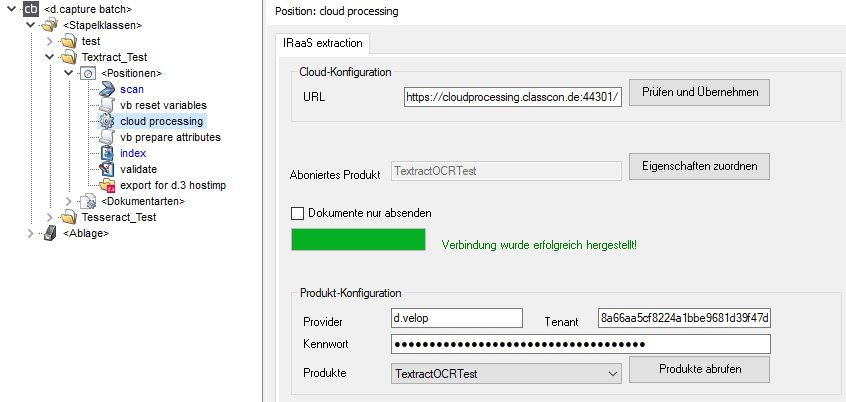
\includegraphics[width=1.1\textwidth]{img/textract_cloudprocessing.png}
    \caption{Einstellung einer Stapelklasse mit Cloud-Processing Position}
    \label{fig-textract-cloudprocessing}
\end{figure}
Die Durchführung der OCR ist eine Position einer Prozess-Sequenz, welche auf dem d.velop Server ausgeführt wird. Eine solche Prozess-Sequenz wird dann von den Kunden abonniert. Neben vordefinierten Prozess-Sequenzen können auch auf Kunden spezifizierte Prozess-Sequenzen angelegt werden.

Bei der OCR-Position kann abermals zwischen ABBYY FineReader und Tesseract ausgewählt werden. Als neue Alternative zu den beiden OCR-Engines (jedoch nur beim Cloud-Processing und nicht bei der lokalen Installation beim Kunden) soll nun noch der neue OCR-Dienst von Amazon Web Services (AWS) eingesetzt werden: Amazon Textract.

Das Angebot von Amazon überzeugt nicht nur preislich, sondern hat auch den Vorteil, dass die eigentliche Texterkennung bei Amazon stattfindet, wodurch die Hardwareanforderungen bei d.velop deutlich sinken. Ein möglicher Geschwindigkeitsverlust wird dabei akzeptiert, da die Cloud-Processing Lösung sowieso nicht schneller sein wird, als eine OCR-Engine die lokal im Kundennetz installiert wurde.
\section{Einführung}
Bevor mit der Programmierung eines Cloud-Dienstes für Amazon Textract begonnen werden kann, sollte geklärt werden, wie die von AWS bereitgestellte API anzusprechen ist. An dieser Stelle sei angemerkt, dass sich Amazon Textract zum Zeitpunkt dieses Praktikums noch in der Testphase befindet. Somit haben sich im Laufe des Praktikums einige Einschränkungen des Dienstes bemerkbar gemacht, auf welche in diesem Bericht noch eingegangen wird. Zum aktuellen Zeitpunkt ist Amazon Textract außerdem nur auf englische Texte ausgelegt.

Amazon Textract ist in der Lage Dokumente sowohl synchron, als auch asynchron zu verarbeiten. Dabei ist zu beachten, dass die synchrone Verarbeitung nur die Bildformate JPG und PNG unterstützt und somit nur Single-Page-Dokumente. Möchte man Multi-Page-Dokumente verarbeiten, so muss eine asynchrone Verarbeitung gestartet werden. Diese unterstützt neben JPG und PNG auch die Verarbeitung von PDF-Dokumenten, was somit schließlich auch das Format für Multi-Page-Dokumente ist. Textract unterscheidet bei der Verarbeitung zwischen reiner Texterkennung (\texttt{TextDetection}) und einer Verarbeitung, die neben der Texterkennung auch noch eine erste semantische Analyse des Textes beinhaltet (\texttt{DocumentAnalysis}). Die Texterkennung liefert für das gesamte Dokument die einzelnen Seiten, Zeilen und Wörter des Textes als sogenannte Blocks. Die Dokumentanalyse liefert neben den reinen Textdaten wahlweise auch noch Key-Value-Paare (z.\,B. Name: Max Mustermann mit Name als Key und Max Mustermann als Value) oder Tabellen und Tabellenzellen mit dem entsprechenden Inhalt. Die möglichen Eigenschaften, die bei der Dokumentanalyse analysiert werden sollen, werden aktiv weiterentwickelt. So ist zum Ende des Praktikums noch die neue Funktion hinzugekommen, dass man bei der Dokumentanalyse auch noch den Namen und Inhalt von Checkboxen und Radiobuttons auslesen lassen kann.
\section{Block-Objekte}
Block-Objekte formen zusammen die Datenstruktur, mit der Textract auf eine Anfrage antwortet. Als Antwort auf eine Anfrage (egal ob reine Texterkennung oder Dokumentanalyse und synchron oder asynchron) wird eine Liste von Block-Objekten zurückgegeben, welche in Leserichtung (von oben nach unten und von links nach rechts) geordnet ist (da Textract zum aktuellen Zeitpunkt nur für englische Dokumente gedacht ist, ist die Leserichtung des Dienstes nicht einstellbar). Auch wenn jeder Block in der API den gleichen Datentyp (\texttt{Block}) besitzt, enthält jeder Block ein \texttt{BlockType} Feld, welches den genauen Blocktypen angibt. Dabei wird unterschieden zwischen \texttt{PAGE}, \texttt{LINE} und \texttt{WORD} (Ergebnisse der Texterkennung), als auch \texttt{KEY\_VALUE\_SET}, \texttt{TABLE} und \texttt{CELL} (Ergebnisse der Dokumentanalyse).

Jeder Block wird in Form einer JSON-Struktur als Antwort übertragen. Die fertige Antwort in der API enthält dann bereits eine Liste von den deserialisierten JSON-Blöcken. Neben den Blöcken enthält die Antwort auch Metadaten, die das gesamte Dokument betreffen (z.\,B. die Anzahl der Seiten). Es folgt eine Übersicht der (relevanten) Felder eines Blocks (dem Feld \texttt{BlockType} ausgeschlossen).
\begin{itemize}
    \item \texttt{Id}: Jeder Block besitzt eine eindeutige Kennung in Form einer Zeichenkette. Diese Id wird genutzt, um die Beziehungen zwischen Blöcken anzugeben.
    \item \texttt{Page}: Die Seitenzahl, auf dem der Inhalt des Blocks zu finden ist.
    \item \texttt{Text}: Der Textinhalt des Blocks (nur für Blöcke der Typen \texttt{LINE} und \texttt{WORD}).
    \item \texttt{Confidence}: Ein Prozentwert, der angibt, wie sicher sich Textract in der Erkennung des Blocks ist.
    \item \texttt{Geometry}: Die Geometrie, die die Position des Blocks auf der Seite angibt. Ein Geometrieobjekt enthält sowohl ein Polygon zur genauen Beschreibung der Geometrie, als auch eine Axis-Aligned-Bounding-Box (AABB) zur groben Beschreibung. Das Polygon besteht aus einer Liste von Punkten mit x- und y-Koordinate, während die AABB die obere linke Ecke und die Breite und Höhe des Rechtecks angibt. Alle Angaben (sowohl die Punkte, also auch die Angaben des Rechtecks) sind Werte aus dem Intervall $[0,1]$ und geben lediglich die relative Position auf der Seite an. Zur Berechnung der absoluten Angaben wird somit die Breite und Höhe der Seite benötigt. Durch die Multiplikation mit der Seitenbreite (für x-Koordinaten und Breitenangaben) bzw. mit der Seitenhöhe (für y-Koordinaten und Höhenangaben) bekommt man somit absolute Werte.
    \item \texttt{Relationships}: Eine Liste von \texttt{Relationship}-Objekten. Aktuell ist diese Liste entweder leer (der Block steht in keiner Beziehung zu anderen Blöcken) oder besitzt exakt ein Element. Dieses \texttt{Relationship}-Objekt besitzt Informationen darüber welche Art von Beziehung vorliegt. Dieser Beziehungstyp ist aktuell entweder \texttt{CHILD}, was eine Parent-Child-Relationship zwischen dem aktuell betrachteten Block und denen im \texttt{Relationship}-Objekt enthaltenen Blöcken darstellt, oder \texttt{VALUE}, wenn der aktuell betrachtete Block ein \texttt{KEY}-Block ist.
    
    Die eigentlichen Blöcke, welche zum betrachteten Block dann in Beziehung stehen, sind im \texttt{Relationship}-Objekt dann als Liste von Strings aufgeführt. Ein Element dieser Liste gibt dann die Id des Child-Blocks als Zeichenkette an.
\end{itemize}
Damit ergibt sich die komplette Struktur eines Dokumentes. Jeder Page-Block einer entsprechenden Seite im Dokument ist die Root-Node eines Baums, der die Struktur dieser Seite beschreibt. Die Child-Nodes eines Page-Blocks sind dann die Zeilen (Line-Block) der entsprechenden Seite. Die Child-Nodes eines Line-Blocks sind letztendlich die Wörter (Word-Block), die in dieser Zeile stehen. Es ergibt sich für jede Seite im Dokument ein (gerichteter) Baum der Maximaltiefe zwei: Die Seite als Root-Node, die Zeilen als Child-Nodes der Seite und die Wörter als Child-Nodes der Zeilen. An dieser Stelle sei noch angemerkt, dass die Reihenfolge der Child-Nodes in einem Block nicht der Leserichtung entspricht (die Child-Nodes und damit Wörter einer Zeile sind somit nicht unbedingt von links nach rechts angeordnet). Die Reihenfolge, in der die Blöcke von Amazon als Antwort zurückkommen, bleibt jedoch weiterhin in Leserichtung.

Die folgende Abbildung zeigt den entstehenden Baum von einem Text, der aus zwei Zeilen besteht.
\begin{figure}[H]
    \centering
    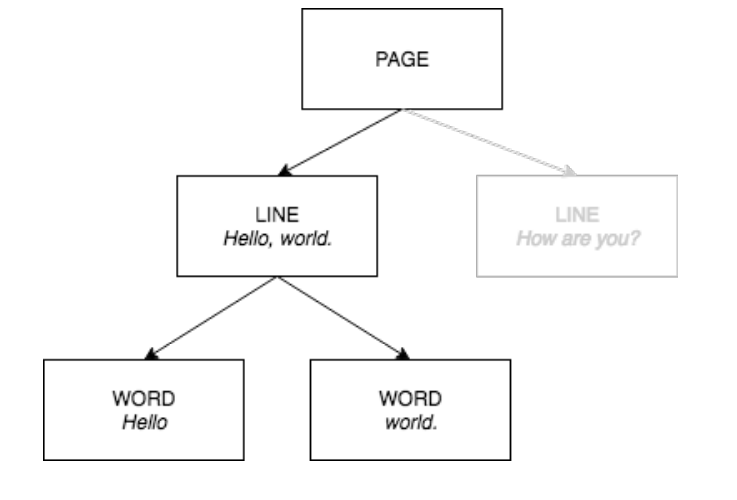
\includegraphics[width=0.7\textwidth]{img/textract_tree.png}
    \caption{Baum von Block-Objekten}
    \label{fig-textract-tree}
\end{figure}
\section{Einrichtung von Amazon Textract in AWS}
Da Amazon Textract zum Zeitpunkt des Praktikums sich noch in der Testphase befindet, haben normale AWS-Accounts standardmäßig keinen Zugriff auf den Dienst. Um an der (geschlossenen) Testphase teilnehmen zu können, muss eine Anfrage auf Teilnahme an Amazon gesendet werden. Sobald der Account dazu berechtigt ist, an der Testphase von Amazon Textract teilzunehmen, muss ein entsprechender Benutzer (IAM User) angelegt werden, der die Rechte bekommt, Amazon Textract zu benutzen. Dies wird im AWS Identity and Access Management (IAM) Dienst konfiguriert. Neben \texttt{AmazonTextractFullAccess} werden auch noch nötige Berechtigungen für Amazon S3 (der Cloudspeicher von AWS), Amazon Simple Queue Service (SQS) und Amazon Simple Notification Service (SNS) gesetzt.

Ist dies erledigt, so kann Amazon Textract bereits mit dem neu angelegten Benutzer ausprobiert werden. Dabei sollte jedoch noch beachtet werden, dass der Dienst in der Testphase nur in eingeschränkten Regionen verfügbar ist. Die einzige Region in Europa, die Textract unterstützt, ist Dublin (Irland).

In der AWS-Konsole lässt sich Amazon Textract mithilfe einer Web-Oberfläche ausprobieren. Im Folgenden wurde eine Beispielrechnung als Bild (PNG-Datei) hochgeladen und ausgewertet.
\begin{figure}[H]
    \centering
    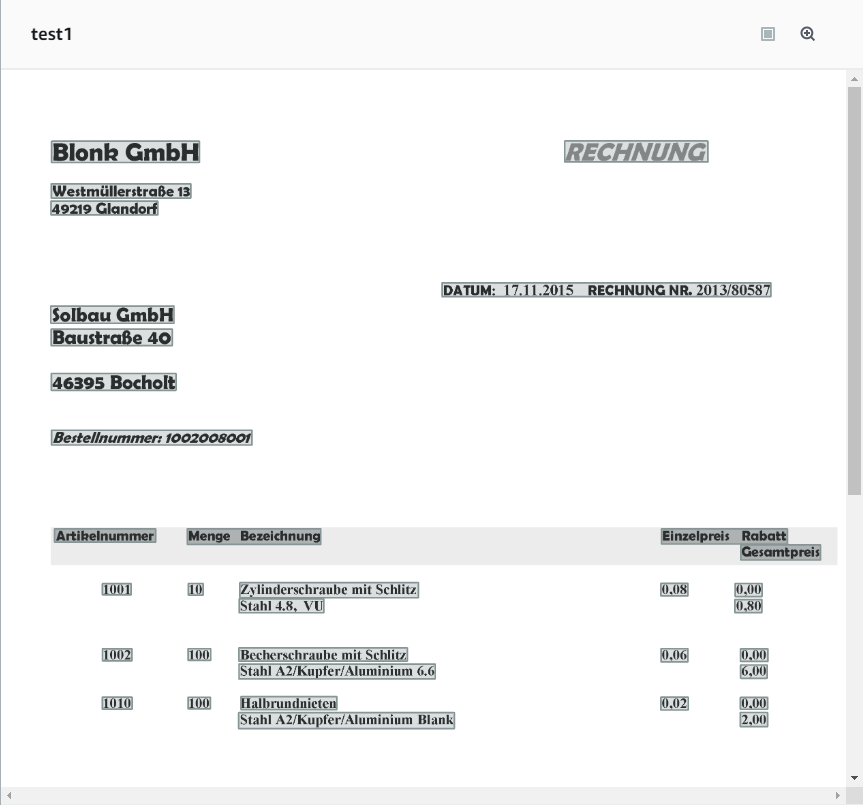
\includegraphics[width=0.7\textwidth]{img/textract_aws_doc.png}
    \caption{Rechnung mit den erkannten Zeilen (grau hinterlegt)}
    \label{fig-textract-aws-doc}
\end{figure}
Als Ausgabe liefert Amazon den erkannten Text, die erkannten Key-Value-Paare und die erkannten Tabellen des Dokumentes. Hier abgebildet ist der erkannte Text (in Form der erkannten Zeilen).
\begin{figure}[H]
    \centering
    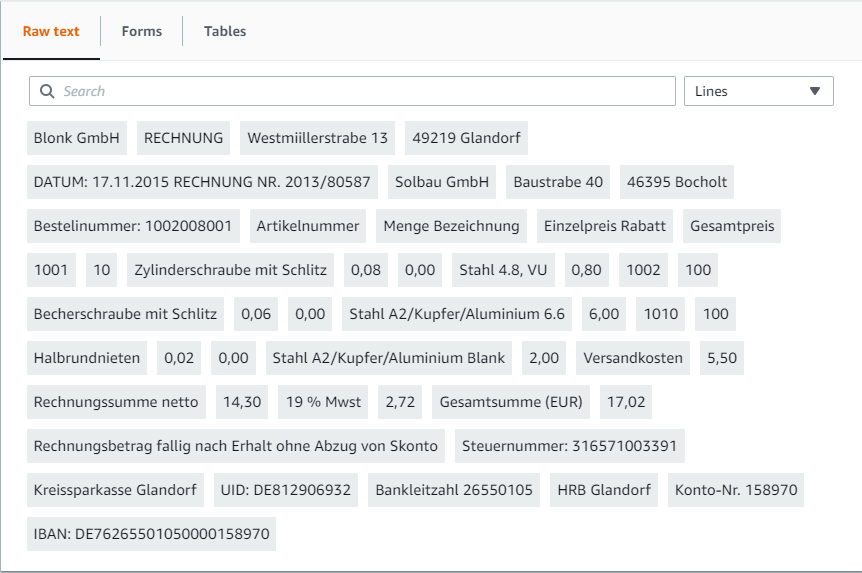
\includegraphics[width=0.8\textwidth]{img/textract_aws_ocr.png}
    \caption{Texterkennung (Zeilen) einer Rechnung}
    \label{fig-textract-aws-ocr}
\end{figure}
Um die API von Amazon Textract nun selber ansprechen zu können, benötigt man zunächst das AWS Command Line Interface (AWS CLI) und ein entsprechendes AWS Software Development Kit (SDK). Da die Software der d.velop AG und damit auch die Software der Classcon Consulting GmbH hauptsächlich in .NET programmiert sind (mit C\# als Programmiersprache), wird das entsprechende AWS SDK für .NET heruntergeladen und eingerichtet. Um das SDK nutzen zu können, wird ein Access-Key benötigt, der für jeden Benutzer neu generiert wird. Es wird also für den zuvor erstellten Benutzer mithilfe der AWS Management Konsole und dem IAM Dienst ein Access-Key generiert. Nach der Installierung des AWS CLI muss dieser Access-Key in die Datei \texttt{C:\textbackslash Users\textbackslash USERNAME\textbackslash .aws\textbackslash credentials} geschrieben werden. Außerdem muss die AWS Region (in unserem Fall Irland - Dublin) gesetzt werden. Dies geschieht in der Datei \texttt{C:\textbackslash Users\textbackslash USERNAME\textbackslash .aws\textbackslash config}. Dublin entspricht der Region \texttt{eu-west-1}.
\section{Limitierungen}
Amazon Textract weist mehrere Limitierungen auf, die auch im Laufe des Praktikums durch diverse Tests aufgefallen sind. Viele dieser Limitierungen gelten jedoch lediglich vorübergehend in der offiziellen Testphase von Textract. Es folgt eine Auflistung dieser nicht änderbaren Limitierungen.
\begin{itemize}
    \item Die maximale Dateigröße für Bilder (JPG oder PNG) beträgt 5 MB.
    \item Die maximale Dateigröße für PDF-Dateien beträgt 500 MB.
    \item Die maximale Anzahl der Seiten einer PDF-Datei beträgt 3000.
    \item Die Minimalhöhe für Text, damit dieser auf einem Dokument erkannt werden kann, beträgt 15 Pixel.
    \item Amazon Textract lässt eine maximale Rotation des Dokumentes von $10\,\%$ zu. Dokumente mit einer schlechteren Ausrichtung können nicht richtig erkannt werden.
    \item Amazon Textract unterstützt keine Handschrifterkennung.
    \item Die synchronen Operationen von Amazon Textract (\texttt{DetectDocumentText} und \texttt{AnalyzeDocument}) unterstützen nur die Bildformate JPG und PNG. Die asynchronen Operationen (\texttt{StartDocumentTextDetection} und \texttt{StartDocumentAnalysis}) unterstützen dazu auch noch PDF-Dateien.
    \item Die maximale Anzahl an asynchronen Jobs, die gleichzeitig bearbeitet werden können ist in der Testphase auf $1$ begrenzt. Es ist also nicht möglich, in der Testphase von Amazon Textract wirklich asynchron zu arbeiten.
    \item Die maximale Anzahl der Transaktionen pro Minute ist in der Testphase auf drei festgelegt.
\end{itemize}
\chapter{Programmierung}
Um sich mit der AWS API vertraut zu machen, wurde zunächst eine Windows-Forms Anwendung entwickelt, die synchrone Texterkennungs- und auch Dokumentanalyse-Anfragen an Amazon stellt. Damit werden zunächst nur Bilder unterstützt. Das Bild wird in der Anwendung dargestellt und die Ergebnisse von Amazon (in Form von Block-Objekten) werden in entsprechenden Tabellen aufgelistet. Eine Interaktion mit einem Block-Objekt (z.\,B. das Markieren einer Zelle einer Tabelle) führt dazu, dass der Inhalt des entsprechenden Blockes im Bild farblich markiert wird.
\section{Synchrone Texterkennung}
Die Dateien, die synchron mit Amazon Textract analysiert werden sollen, können entweder in Amazon S3-Buckets abgelegt werden und dann mit dem entsprechenden Namen in der Anfrage referenziert werden oder man überträgt ein Bild als Base64-codiertes Byte-Array. Dieses Byte-Array kann dann direkt als Eingabeparameter der Anfrage mitgegeben werden. Da zunächst nur die Funktionsweise des Dienstes getestet werden sollte, werden die Dokumente nicht nach Amazon S3 hochgeladen, sondern einfach als Byte-Array nach Amazon gesendet.

Als Anfrage wird \texttt{AnalyzeDocument} verwendet, womit neben dem reinen Text (Zeilen und Wörter) auch noch Formulardaten (Key-Value-Paare) und Tabellen (mit ihren Zellen) als Antwort zurückgegeben werden (dazu wird beim \texttt{AnalyzeDocumentRequest} als \texttt{FeatureTypes} \texttt{FORMS} und \texttt{TABLES} angegeben).
\begin{figure}[H]
    \centering
    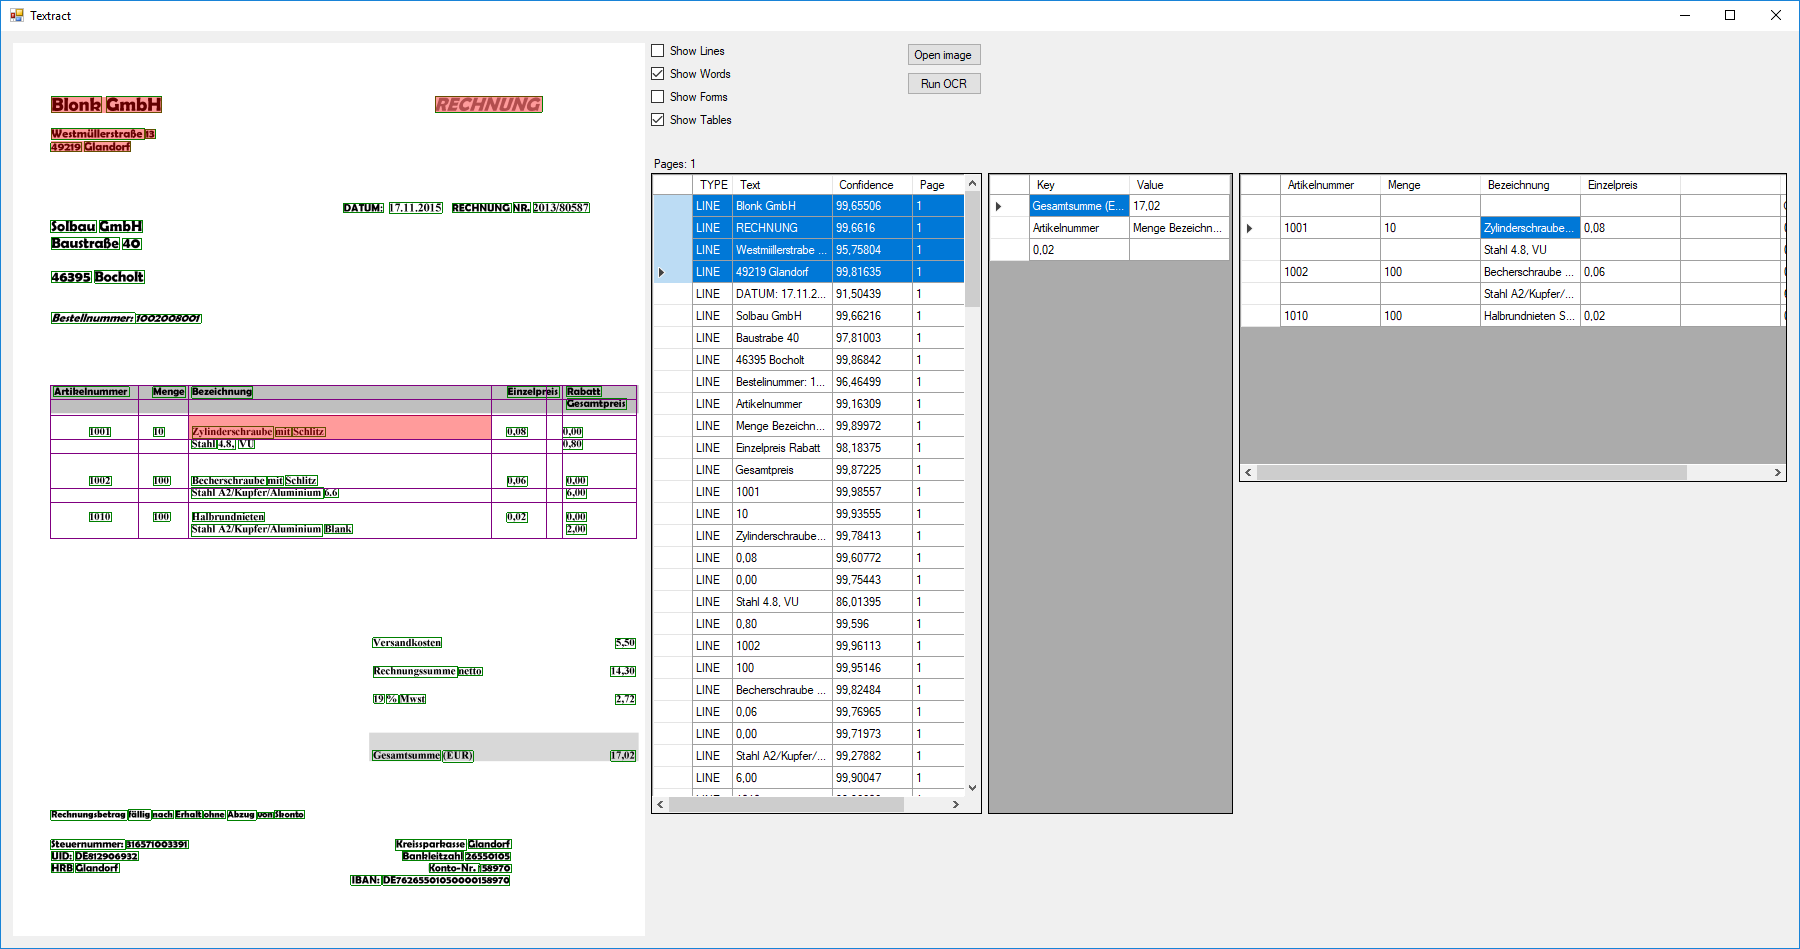
\includegraphics[width=1.0\textwidth]{img/textract_gui.png}
    \caption{Auswertung eines Dokumentes mit Textract API}
    \label{fig-textract-gui}
\end{figure}
Die Abbildung zeigt die Auswertung eines Dokumentes in der selbst programmierten Textract GUI. Die AABBs der vier verschiedenen Blocktypen (Zeilen, Wörter, Formulardaten und Tabellen) lassen sich per Checkboxen anzeigen. Um die Geometrie einzelner markierter Blöcke hervorheben zu können, werden die Blöcke bei der Auswertung der OCR-Antwort in ein \texttt{Dictionary} gespeichert (so wird in C\# eine generische \texttt{HashMap} bezeichnet), welches die Block-Id (ein String) auf das entsprechende Block-Objekt abbildet. Die jeweilige Block-Id eines Objektes wird in der GUI versteckt hinterlegt (als Eigenschaft einer Zeile oder Zelle der Tabellen). Damit lässt sich das Objekt bei Markierung in durchschnittlich konstanter Zeit direkt farbig hervorheben.
\section{Asynchrone Texterkennung}
Da der zu programmierende Dienst natürlich auch mehrseitige Dokumente unterstützen soll, wurde sich noch mit der asynchronen Texterkennung beschäftigt. Dazu wurde zunächst die eigene GUI soweit erweitert, dass diese asynchrone Anfragen an Amazon stellt.

Da nicht alle Dokumente der Classcon Consulting GmbH im PDF-Format sind (das einzige mehrseitige Format, was von Amazon Textract unterstützt wird), sondern viele im TIF-Format sind, wurde zunächst eine Methode geschrieben, welche TIF-Dateien in PDF-Dateien umwandelt.

Dokumente, die asynchron verarbeitet werden sollen, müssen in Amazon S3-Buckets liegen. Damit muss jedes Dokument vor der Texterkennung in einen solchen Bucket hochgeladen werden und am Ende sollte das Dokument auch wieder aus dem Bucket entfernt werden. Die asynchronen Klassen der Textract API weisen den Präfix \texttt{Start} auf, somit ist der asynchrone Request auf eine Texterkennung mit der Klasse \texttt{StartDocumentTextDetectionRequest} möglich. Sobald dieser Request fertig abgearbeitet wurde von Amazon, wird eine entsprechende Nachricht in ein (zuvor angelegtes) Amazon SNS Topic bekannt gegeben. Dieses Topic lässt sich mit einer Amazon SQS Queue überwachen (die Queue \textit{abonniert} das Topic). Die Nachricht lässt sich dann aus der Queue herauslesen. Bei einer erfolgreichen Verarbeitung findet sich in den Metadaten dann eine eindeutige \texttt{JobId}, welche als Parameter für einen \texttt{GetDocumentTextDetectionRequest} verwendet wird. Damit lässt sich das eigentliche Ergebnis der Texterkennung abfragen.

Folgender Ausschnitt an C\# Code zeigt die grobe Vorgehensweise bei der asynchronen Texterkennung mit Amazon Textract.
\begin{lstlisting}[caption=Asynchrone Texterkennung in Amazon Textract, label=lst:textract_async]
using (var textractClient = new AmazonTextractClient(
    ACCESS_KEY_ID,
    SECRET_ACCESS_KEY,
    RegionEndpoint.EUWest1
))
using (var sqsClient = new AmazonSQSClient(
    ACCESS_KEY_ID,
    SECRET_ACCESS_KEY,
    RegionEndpoint.EUWest1
))
{
    var startResp = textractClient.StartDocumentTextDetection(
        new StartDocumentTextDetectionRequest {
            DocumentLocation = new DocumentLocation {
                S3Object = new S3Object {
                    Bucket = BUCKET_NAME,
                    Name = fileToOCR
                }
            }, NotificationChannel = new NotificationChannel {
                RoleArn = ROLE_ARN,
                SNSTopicArn = TOPIC_ARN
            }
        }
    );
    
    bool jobFound = false;
    do
    {
        foreach (var msg in sqsClient.ReceiveMessage(QUEUE_URL).Messages)
        {
            var body = JsonConvert.DeserializeObject<dynamic>(msg.Body);
            var message = JsonConvert.DeserializeObject<dynamic>(body.Message);
            var jobId = message.JobId;
            var status = message.Status;

            if (jobId == startResp.JobId)
            {
                jobFound = true;

                if (status == "SUCCEEDED")
                {
                    string token = null;
                    do
                    {
                        var getResp = textractClient.GetDocumentTextDetection(
                            new GetDocumentTextDetectionRequest {
                                JobId = jobId,
                                NextToken = token
                            }
                        );

                        foreach (var block in getResp.Blocks)
                        {
                            // Process block
                        }

                        token = getResp.NextToken;
                    } while (token != null);
                }

                sqsClient.DeleteMessage(QUEUE_URL, msg.ReceiptHandle);
                break;
            }
        }
    } while (!jobFound);
}
\end{lstlisting}
\section{Cloud-Dienst}
Die Aufgabe des Dienstes ist es, für ausstehende Dokumente eine OCR durchzuführen und das Ergebnis der Texterkennung in eine XML-Struktur zu schreiben, welche dann später zur Klassifizierung wieder eingelesen und ausgewertet wird. Der Dienst arbeitet dabei mit mehreren Threads (jeder Thread übernimmt die Texterkennung eines Dokumentes), deren Anzahl konfigurierbar ist und standardmäßig zwischen (einschließlich) $2$ und $5$ liegt.

Die betriebsinterne XML-Struktur, welche den erkannten Text eines Dokumentes speichert, ist dabei hierarchisch aufgebaut: Unter der Parent-Node befindet sich für jede Seite eine Page-Node mit Metadaten zur Seite (Seitenzahl, Höhe und Breite der Seite) und zwei weiteren Attributen, die den Inhalt der Seite beschreiben. Das erste Attribut enthält eine Aufzählung von Unicode Werten, welche letztendlich den kompletten Text der Seite ergeben. Das zweite Attribut beschreibt für jedes Unicode Zeichen das Rechteck (Left, Top, Width, Height), welches die Position des Zeichens auf der Seite angibt.

Die Vorgehensweise des Dienstes (bzw. jedes Threads des Dienstes) kann dabei folgendermaßen beschrieben werden: Sofern ein Dokument zur Texterkennung aussteht, wird zunächst sichergestellt, dass die Datei vom Dateityp PDF ist (im Falle einer TIF-Datei wird diese in eine PDF-Datei umgewandelt). Daraufhin wird die Datei mit einem Globally Unique Identifier (GUID) versehen, damit sichergestellt wird, dass der Dateiname eindeutig ist. Die Datei wird in einen Amazon S3-Bucket hochgeladen und es wird eine asynchrone Texterkennungsanfrage (keine Dokumentanalyse, da wir nur Seiten, Zeilen und Wörter benötigen) an Textract gestellt. Es werden für jeden Page-Block in der XML-Struktur ein neues Page-Element angelegt und danach jeder Line-Block der Seite durchgegangen und der Unicode-Wert jedes Zeichens der Zeile notiert. Die Geometrie (das Rechteck) der Zeile wird gleichmäßig auf die Anzahl der Zeichen in der Zeile aufgeteilt, da Textract leider keine Möglichkeit bietet, das Rechteck eines einzelnen Zeichens abzufragen. Am Ende wird das Dokument im S3-Bucket wieder gelöscht und das Ergebnis der OCR (in Form der XML-Struktur) wird lokal gespeichert.
\chapter{Statistische Auswertung}
Da Amazon Textract als Alternative zu ABBYY FineReader oder Tesseract OCR eingesetzt werden soll, soll sowohl die Geschwindigkeit als auch die Erkennungsqualität des Dienstes ausgewertet und bewertet werden.
\section{Geschwindigkeit}
Da es zum Zeitpunkt des Praktikums leider nicht möglich ist, Dokumente in Textract parallel auszuwerten (da die Anzahl asynchroner Jobs auf $1$ limitiert ist), lässt sich noch keine Aussage über die Skalierbarkeit des Dienstes treffen. Die durchschnittliche Auswertungszeit eines Dokumentes mit nur einer Seite (inklusive dem Hochladen nach Amazon S3 und dem Erstellen der XML-Struktur) beträgt etwa $7$ Sekunden. Diese Zeit ist zwar schlechter als die von ABBYY FineReader (etwa $4$ Sekunden) und Tesseract OCR (etwa $5$ Sekunden), gilt aber trotzdem als akzeptabel. Dies ist damit zu begründen, dass die anderen beiden Dienste lokal (also im auf Servern im betriebsinternen Netzwerk) laufen, während die Kommunikation mit Textract über entfernte Amazon Server geht. Da Textract zudem in der Testphase in EU nur in Dublin (Irland) unterstützt wird, ist der Kommunikationsweg noch länger als er im normalen Fall (mit Frankfurt als Region) sein sollte.
\section{Erkennungsqualität}
Um die Erkennungsqualität von Amazon Textract bewerten zu können, werden $1.157$ Beispielrechnungen eingelesen und deren Rechnungsnummern extrahiert. Die extrahierte Rechnungsnummer wird mit der korrekten Rechnungsnummer (welche sich in einer Datenbank befindet) abgeglichen. Es wird sich dabei zunächst auf die Auswertung der Rechnungsnummer beschränkt, da Amazon Textract zum aktuellen Zeitpunkt noch keinen deutschen Wörterbuchabgleich durchführt und lediglich deutsche Beispieldokumente zum Testen vorhanden sind. Damit würde Amazon Textract bei deutschen Texten aktuell sicherlich schlechtere Ergebnisse liefern, als ABBYY FineReader oder Tesseract OCR (welche beide einen Abgleich mit bekannten deutschen Wörtern durchführen). Da die Rechnungsnummern der Dokumente hauptsächlich aus zusammenhangslosen Zeichenketten (Buchstaben, Zahlen und gelegentlich auch Sonderzeichen) bestehen, würde ein Wörterbuchabgleich an dieser Stelle keine Vorteile geben.

Zum Vergleich der ausgelesenen Rechnungsnummern mit den korrekten Rechnungsnummern ist eine Metrik notwendig, die angibt, wie ähnlich oder unterschiedlich zwei Zeichenketten voneinander sind. Wir betrachten dafür die Editierdistanz.
\subsection{Editierdistanz}
Die Editierdistanz ist eine Metrik, die angibt wie unterschiedlich zwei Strings (Zeichenketten) voneinander sind, indem die kleinste Anzahl der nötigen Editierungsoperationen gezählt wird, welche einen String in einen anderen String transformieren. Die genaue Definition der Editierdistanz hängt davon ab, welche Art von Operationen zur Editierung zugelassen sind. Unter solchen Operationen zählen das Entfernen von einem Zeichen (\texttt{Deletion}), das Einfügen von einem Zeichen (\texttt{Insertion}), das Ersetzen von einem Zeichen durch ein anderes Zeichen (\texttt{Substitution}) und auch das Vertauschen zweier aneinanderliegender Zeichen (\texttt{Transposition}). Wir betrachten im Folgenden hauptsächlich die Levenshtein-Distanz, welche als Operationen das Entfernen, Einfügen und Ersetzen von einem Zeichen im String zulässt.

Wir legen dabei die Kosten jeder Operation auf $1$ fest, womit die minimale Distanz also die minimale Anzahl an nötigen Operationen wird. Eine allgemeinere Definition würde jede Operation mit eigenen (nicht negativen) Kosten versehen ($C_{del},C_{ins},C_{sub}$).
\subsection{Levenshtein-Distanz}
Für zwei Zeichenfolgen $a,b$ mit entsprechenden Längen $|a|,|b|$ weist die Levenshtein-Distanz $d(a,b)$ dann unter anderem folgende Eigenschaften auf:
\begin{itemize}
    \item $a=b\Longleftrightarrow d(a,b)=0$, da jeder String ohne Operationen in sich selber transformierbar ist.
    \item $a\neq b\Longleftrightarrow d(a,b)>0$, da mindestens eine Operation (mit nicht negativen Kosten) nötig ist, um $a$ in $b$ zu transformieren.
    \item $d(a,b)=d(b,a)$, da die Kosten zum Entfernen und zum Einfügen eines Zeichens gleich sind und die beiden Operationen die inverse Operation der jeweils anderen darstellen.
    \item $d(a,b)+d(b,c)\geq d(a,c)$ (Dreiecksungleichung), da $b$ im besten Fall ein Zwischenschritt in der Transformation von $a$ nach $c$ ist, kann die linke Seite der Ungleichung nicht kleiner als $d(a,c)$ sein.
    \item $d(a,b)\geq||a|-|b||$, da bei der Transformation $a$ auf die Länge von $b$ gebracht werden muss und dabei mindestens $||a|-|b||$ Operationen (Entfernen oder Einfügen, je nachdem welcher String länger ist) nötig sind.
    \item $d(a,b)\leq \max(|a|,|b|)$, da im schlechtesten Fall (keine Zeichen aus $a$ lassen sich zu $b$ zuordnen) $\min(|a|,|b|)$ Zeichen durch andere ersetzt werden müssen und die weiteren $\max(|a|,|b|)-\min(|a|,|b|)$ Zeichen entweder entfernt oder eingefügt werden müssen (je nachdem welcher String länger ist).
\end{itemize}
Die Levenshtein-Distanz zwischen dem Wort \texttt{levenshtein} und dem Wort \texttt{meilenstein} (bei uniformen Operationskosten von $1$) ist $4$. Eine mögliche Umwandlung von \texttt{levenshtein} nach \texttt{meilenstein} könnte zum Beispiel folgendermaßen aussehen:
\begin{enumerate}
    \item \texttt{\textbf{l}evenshtein} $\rightarrow$ \texttt{\textbf{m}evenshtein} (Ersetzen von \texttt{l} durch \texttt{m})
    \item \texttt{me\textbf{v}enshtein} $\rightarrow$ \texttt{me\textbf{i}enshtein} (Ersetzen von \texttt{v} durch \texttt{i})
    \item \texttt{meienshtein} $\rightarrow$ \texttt{mei\textbf{l}enshtein} (Einfügen von \texttt{l})
    \item \texttt{meilens\textbf{h}tein} $\rightarrow$ \texttt{meilenstein} (Entfernen von \texttt{h})
\end{enumerate}
Mit den Strings $a=a_1\dots a_{|a|}$ und $b=b_1\dots b_{|b|}$ folgt die rekursive Definition der Levenshtein-Distanz. Dabei steht $d(i,j)$ für die Levenshtein-Distanz zwischen den ersten $i$ Zeichen von $a$ und den ersten $j$ Zeichen von $b$.
\begin{align}
    d(i,j)=\begin{cases}
        j & i=0\\
        i & j=0\\
        \min\begin{cases}
            d(i-1,j-1)+[a_i\neq b_j]\\
            d(i,j-1)+1\\
            d(i-1,j)+1
        \end{cases} & 1\leq i\leq |a| \wedge 1\leq j\leq |b|
    \end{cases}
\end{align}
Die Levenshtein-Distanz der beiden kompletten Strings ist dann gegeben durch $d(|a|,|b|)$. Außerdem sei angemerkt, dass das erste Element im Minimum der Substitution eines Zeichens entspricht (bzw. der Zuordnung zweier Zeichen, sofern diese gleich sind), wobei $[a_i\neq b_j]$ für das Iverson-Bracket steht, welches zu $1$ evaluiert, sofern der Ausdruck in den Klammern wahr ist und zu $0$ wenn der Ausdruck unwahr ist. Das zweite Element im Minimum steht für das Einfügen eines Zeichens in $a$ (wir betrachten die Operationen weiterhin von $a$ nach $b$) und das dritte Element steht für das Entfernen eines Zeichens aus $a$. Die Basisfälle der Rekursion berechnen die Distanz mit einem leeren String. Da wir für das Einfügen und für das Entfernen eines Zeichens jeweils die Kosten $1$ haben gilt für jeden String $s$: $d(s,\varnothing)=d(\varnothing,s)=|s|$. Anschaulich ist dies damit zu begründen, dass ein leerer String durch das Einfügen von exakt $|s|$ Zeichen in einen String $s$ transformiert werden kann und umgekehrt kann jeder String $s$ durch das Entfernen von exakt $|s|$ Zeichen in den leeren String transformiert werden.

An dieser Stelle kann mithilfe einer weiteren Eigenschaft der Editierdistanz eine erste Optimierung vorgenommen werden. Wenn die Strings $a$ und $b$ einen gemeinsamen Präfix besitzen, dann ist dieser Präfix für die Berechnung der Editierdistanz $d(a,b)$ nicht relevant. Für jeden Präfix $u$ gilt somit $d(ua,ub)=d(a,b)$. Für unseren rekursiven Algorithmus bedeutet dies, dass im Falle von $a_i=b_j$ die Distanz $d(i,j)$ direkt als $d(i-1,j-1)$ berechnet werden kann, wodurch an dieser Stelle zwei rekursive Aufrufe gespart werden. Der Algorithmus sieht dann folgendermaßen aus:
\begin{align}
    d(i,j)=\begin{cases}
        j & i=0\\
        i & j=0\\
        \begin{cases}
            d(i-1,j-1) & a_i=b_j\\
            1+\min\begin{cases}
                d(i-1,j-1)\\
                d(i,j-1)\\
                d(i-1,j)
            \end{cases} & a_i\neq b_j
        \end{cases} & 1\leq i\leq |a| \wedge 1\leq j\leq |b|
    \end{cases}
\end{align}
Der Algorithmus kann direkt nach der obigen Formulierung rekursiv implementiert werden.

Es folgt eine Implementation in C\#, wobei der eigentliche Algorithmus als private Methode implementiert wurde (damit diese durch die Indizes rekursionsfähig ist). Eine weitere öffentliche Methode stellt die Schnittstelle zum Programmierer dar. Diese ruft den Algorithmus mit $i=|a|$ und $j=|b|$ auf und berechnet somit mit $d(|a|,|b|)$ die Editierdistanz zwischen allen Zeichen von $a$ und allen Zeichen von $b$.
\begin{lstlisting}[caption=Rekursiver Algorithmus zur Berechnung der Levenshtein-Distanz, label=lst:levenshtein_recursive]
private static int LevenshteinDistance(string a, string b,
                                       int    i, int    j)
{
    if (i == 0) return j;
    if (j == 0) return i;

    // Subtraktion von 1 im Index, da nullbasierte Strings
    if (a[i - 1] == b[j - 1])
    {
        return LevenshteinDistance(a, b, i - 1, j - 1);
    }

    return 1 + Math.Min(
        LevenshteinDistance(a, b, i - 1, j - 1), // Substitution
        Math.Min(
            LevenshteinDistance(a, b, i, j - 1), // Insertion
            LevenshteinDistance(a, b, i - 1, j)  // Deletion
        )
    );
}

public static int LevenshteinDistance(string a, string b)
{
    return LevenshteinDistance(a, b, a.Length, b.Length);
}
\end{lstlisting}
\subsection{Dynamische Programmierung}
Leider ist dieser rekursive Ansatz nicht sehr effizient. Um dies zu verdeutlichen betrachten wir die ersten beiden Rekursionstiefen des Algorithmus bei der Berechnung einer Distanz $d(i,j)$. Wir gehen dabei von dem schlechten Fall aus, dass keine Zeichen übereinstimmen und wir immer alle drei Fälle für das Minimum auswerten müssen. Die Reihenfolge, in der die drei Fälle ausgewertet werden bleiben weiterhin zunächst Substitution, dann Insertion und zuletzt Deletion (dies dient jedoch nur zur weiteren Erklärung).
\begin{figure}[H]
    \centering
    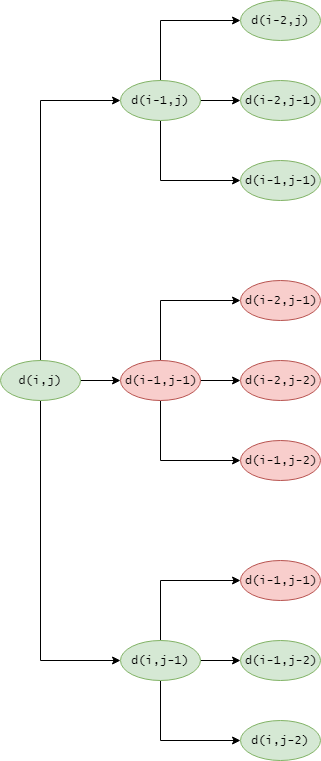
\includegraphics[width=0.6\textwidth]{img/levenshtein_recursion.png}
    \caption{Rekursionsbaum bei der Berechnung der Levenshtein-Distanz}
    \label{fig-levenshtein-recursion}
\end{figure}
Wie zu erkennen ist, werden die gleichen Teilprobleme von $d(i,j)$ mehrmals berechnet ($d(i-1,j-1)$ würde dreimal berechnet werden). Diese kombinatorische Explosion führt zu einem exponentiellen Laufzeitverhalten von $\Omega(3^{\min(|a|,|b|)})$ und $\mathcal{O}(3^{|a|+|b|})$. Außerdem sei angemerkt, dass der Algorithmus (auch wenn nicht explizit Speicher angelegt wird) durch den Aufbau des Stacks bei der Rekursion eine Speicherkomplexität von $\Theta(|a|+|b|)$ besitzt, da die längsten Wege durch den Rekursionsbaum von $d(|a|,|b|)$ nach $d(0,0)$, $d(0,1)$ oder $d(1,0)$ gehen ohne dabei den Rekursionsschritt $d(i-1,j-1)$ zu benutzen, wobei exakt $|a|+|b|$ Funktionsaufrufe des Algorithmus auf dem Stack liegen.

Dies ist ein klassisches Problem aus der dynamischen Programmierung (DP). Der erste Lösungsansatz wäre es, den rekursiven Algorithmus so anzupassen, dass jedes Teilproblem nur einmal berechnet wird, gespeichert wird und im Verlauf der weiteren Rekursion jederzeit wieder abgerufen werden kann. Somit wird nicht unnötig wieder tiefer in die Rekursion gegangen und das Ergebnis kann direkt zurückgegeben werden. Diese Technik wird in der Literatur als Memoisation bezeichnet. Als Datenstruktur für die Memoisation benötigen wir hier ein zweidimensionales Array der Dimension $|a|\times |b|$, für alle möglichen Ergebnisse von $d(i,j):1\leq i\leq|a|,1\leq j\leq|b|$.

Da Rekursion zunächst in die Tiefe geht, bevor das nächste Teilproblem eines Rekursionslevels abgearbeitet wird, ergibt sich eine Arbeitsweise wie in der Abbildung \ref{fig-levenshtein-recursion} gezeigt. Die grünen Aufrufe werden berechnet und für den weiteren Verlauf zwischengespeichert. Die roten Aufrufe sind Teilprobleme, die bereits berechnet wurden und gehen damit nicht weiter in die Rekursion, sondern geben lediglich den bereits berechneten Wert zurück. In der Abbildung wird $d(i-1,j-1)$ zunächst als Teilproblem von $d(i-1,j)$ berechnet (was wiederum ein Teilproblem von unseren initialen Problem $d(i,j)$ ist). Nachdem $d(i-1,j)$ komplett berechnet wurde, würde der Algorithmus auf dem höchsten Rekursionslevel zurückkehren und probieren mit $d(i-1,j-1)$ weiter zu machen. Da dieses Problem jedoch bereits berechnet wurde, wird der komplette Rekursionszweig abgeschnitten und es wird nur der zuvor berechnete Wert zurückgegeben.

Eine mögliche Umsetzung in C\# könnte folgendermaßen aussehen:
\begin{lstlisting}[caption=Levenshtein-Distanz mit Memoisation, label=lst:levenshtein_memoization]
private static int LevenshteinDistance(string a, string b, int i, int j, int[,] memo)
{
    if (memo[i, j] > -1)
    {
        // Rueckgabe des bereits berechneten Wertes
        return memo[i, j];
    }

    // Sonst Wert normal berechnen, speichern und zurueckgeben
    if (i == 0) return memo[i, j] = j;
    if (j == 0) return memo[i, j] = i;

    if (a[i - 1] == b[j - 1])
    {
        memo[i, j] = LevenshteinDistance(a, b, i - 1, j - 1, memo);
    }
    else
    {
        memo[i, j] = 1 + Math.Min(
            LevenshteinDistance(a, b, i - 1, j - 1, memo),
            Math.Min(
                LevenshteinDistance(a, b, i, j - 1, memo),
                LevenshteinDistance(a, b, i - 1, j, memo)
            )
        );
    }

    return memo[i, j];
}

public static int LevenshteinDistance(string a, string b)
{
    // (|a| + 1) x (|b| + 1) Array um die Basisfaelle mitzuspeichern
    // Vereinfacht auch den Umgang mit den einsbasierten Indizes
    int[,] memo = new int[a.Length + 1, b.Length + 1];

    // Memotable mit Wert fuellen, der als "nicht berechnet" gilt
    for (int i = 0; i <= a.Length; i++)
    {
        for (int j = 0; j <= b.Length; j++)
        {
            memo[i, j] = -1;
        }
    }

    return LevenshteinDistance(a, b, a.Length, b.Length, memo);
}
\end{lstlisting}
Der Ansatz mit Memoisation weist nun zwar eine höhere Speicherkomplexität von $\Theta(|a|\cdot|b|)$ auf (dieser Speicher wird benötigt, um die Ergebnisse der Teilprobleme zwischenzuspeichern), besitzt aber dafür auch eine Laufzeitkomplexität von $\Theta(|a|\cdot|b|)$, da jedes der $|a|\cdot|b|$ Teilprobleme nur noch einmal berechnet werden muss und nicht mehr als $3$ mal sein Ergebnis zurückgeben muss.

Da dieser Top-down-Ansatz (wir starten beim Ausgangsproblem $d(|a|,|b|)$ und gehen in der Rekursion bis zu den Basisfällen) weiterhin auf Rekursion basiert, wird für die Erhaltung des Rekursionsstacks zusätzlicher Speicher und Leistung (Auf- und Abbau des Stacks) aufgebracht. Wir betrachten damit noch eine finale Lösung, welche auch auf DP basiert, aber iterativ arbeitet.

Alternativ zur vorherigen Lösung füllen wir unser DP-Array nun nach dem Bottom-up-Ansatz: Wir tragen die Werte für die Basisfälle $d(0,j)$ und $d(i,0)$ direkt ein und gehen die Teilprobleme dann so durch, dass diese sofort mit den Ergebnissen der vorherigen Teilprobleme berechnet werden können. Dazu berechnen wir zunächst die Teilprobleme $d(1,j)$ für $j=1\mathinner{\ldotp\ldotp}|b|$. Die aufsteigende Reihenfolge für $j$ ist dabei wichtig, da wir für die Berechnung von $d(1,j)$ das Ergebnis von $d(1,j-1)$ benötigen (für $j=1$ ist dies kein Problem, da wir $d(i,0)$ für alle $i$ bereits eingetragen haben). Da wir auch die Ergebnisse aller $d(0,j)$ schon haben, können wir damit nun alle $d(1,j)$ berechnen. Mit allen $d(1,j)$ können wir dann aber alle $d(2,j)$ berechnen. Allgemein benötigen wir alle $d(i-1,j)$ um alle $d(i,j)$ zu berechnen. Für alle $i=1\mathinner{\ldotp\ldotp}|a|$ (wieder aufsteigende Reihenfolge) berechnen wir also mit $j=1\mathinner{\ldotp\ldotp}|b|$ alle $d(i,j)$ ohne dabei auf Teilprobleme zu stoßen, die wir für $d(i,j)$ benötigen aber noch nicht berechnet haben. Am Ende ist $i=|a|$ und $j=|b|$ und wir berechnen das Ergebnis des Ausgangsproblems $d(|a|,|b|)$.

Dieser Algorithmus zur Berechnung der Levenshtein-Distanz wird auch als Wagner-Fischer-Algorithmus bezeichnet. Der Algorithmus wurde auch folgendermaßen in C\# implementiert, um die Editierdistanz zwischen zwei Rechnungsnummern zu finden.
\begin{lstlisting}[caption=Wagner-Fischer-Algorithmus, label=lst:wagner_fischer]
public static int WagnerFischer(string a, string b)
{
    int m = a.Length;
    int n = b.Length;

    int[,] d = new int[m + 1, n + 1];

    // Basisfaelle eintragen
    for (int i = 0; i <= m; i++) d[i, 0] = i;
    for (int j = 0; j <= n; j++) d[0, j] = j;

    for (int i = 1; i <= m; i++)
    {
        for (int j = 1; j <= n; j++)
        {
            if (a[i - 1] == b[j - 1])
            {
                d[i, j] = d[i - 1, j - 1];
            }
            else
            {
                d[i, j] = 1 + Math.Min(
                    d[i - 1, j - 1],
                    Math.Min(
                        d[i, j - 1],
                        d[i - 1, j]
                    )
                );
            }
        }
    }

    // Ergebnis steht in d(m, n) = d(|a|, |b|)
    return d[m, n];
}
\end{lstlisting}
Die Laufzeitkomplexität des Wagner-Fischer-Algorithmus beträgt wie auch beim Top-down-Ansatz $\Theta(|a|\cdot|b|)$. Der abgebildete Algorithmus besitzt auch weiterhin eine Speicherkomplexität von $\Theta(|a|\cdot|b|)$. Dies lässt sich jedoch noch verbessern, wenn man beachtet, dass für die Berechnung von $d(|a|,|b|)$ nicht die komplette Matrix aufgebaut werden muss. Stattdessen reicht es nur zwei Zeilen zu speichern (die zuvor berechnete Zeile und die aktuelle Zeile). Dies lässt sich damit begründen, dass für eine Zeile $i$ der Matrix, zur Berechnung aller Distanzen $d(i,j)$ dieser Zeile nur die Werte aus den vorherigen Berechnungen $d(i-1,j)$ benötigt werden (für Substitution und Deletion) und der Wert direkt links (in derselben Zeile) vom aktuell berechneten Wert (für Insertion). Die Distanzen $d(u,j)$ mit $u<i-1$ sind also für die weiteren Berechnungen nicht mehr relevant und müssen nicht gespeichert werden. Wählt man nun die Länge des kürzeren Strings als Dimension dieser Zeile werden exakt zwei Arrays der Größe $\min(|a|,|b|)$ benötigt. Damit ergibt sich eine verbesserte Speicherkomplexität von $\Theta(\min(|a|,|b|))$. Dies lässt sich noch weiter verbessern auf nur eine Zeile und eine Variable, da für die Berechnung von $d(i,j)$ auch alle $d(i-1,v)$ mit $v<j-1$ irrelevant sind. Wir überschreiben also die Werte der alten Zeile mit den neu berechneten Werten. Dabei steht (der bereits neue Wert) $d(i,j-1)$ direkt links in der Zeile, der alte Wert $d(i-1,j)$ steht noch an der Stelle, wo jetzt der neue Wert $d(i,j)$ reingeschrieben wird. Die zusätzliche Variable speichert $d(i-1,j-1)$, dessen Wert zuvor links vom aktuellen Wert stand, jedoch durch den Wert $d(i,j-1)$ überschrieben wurde. Vor jedem Überschreiben eines Wertes müssen wir also den alten Wert zwischenspeichern, da dieser Wert im nächsten Schritt noch mal gebraucht wird.

Die speicheroptimierte Version des Wagner-Fischer-Algorithmus sieht folgendermaßen in C\#-Code aus:
\begin{lstlisting}[caption=Wagner-Fischer-Algorithmus mit Speicheroptimierung, label=lst:wagner_fischer_space]
public static int WagnerFischerSpaceOptimization(string a,
                                                 string b)
{
    int m = a.Length;
    int n = b.Length;

    // Speicherkomplexitaet von O(min(|a|,|b|)) sicherstellen
    if (m < n) return WagnerFischerSpaceOptimization(b, a);

    int[] d = new int[n + 1];
    for (int j = 0; j <= n; j++) d[j] = j;

    for (int i = 1; i <= m; i++)
    {
        int diag = d[0]; d[0] = i;
        for (int j = 1; j <= n; j++)
        {
            int tmp = d[j];
            if (a[i - 1] == b[j - 1])
            {
                d[j] = diag;
            }
            else
            {
                d[j] = 1 + Math.Min(
                    diag,
                    Math.Min(
                        d[j - 1],
                        d[j]
                    )
                );
            }
            diag = tmp;
        }
    }

    return d[n];
}
\end{lstlisting}
Der Nachteil bei der speicheroptimierten Version ist, dass am Ende des Algorithmus nicht noch mal die Matrix durchlaufen werden kann, um nachzuvollziehen, welche Operationen zu der minimalen Editierdistanz führen. Wir betrachten dazu noch mal das Beispiel mit $a="levenshtein"$ und $b="meilenstein"$ und einer Editierdistanz von $4$ (vgl. Abb. \ref{fig-levenshtein-backtracking}).

Möchten wir nun zusätzlich zu der Editierdistanz noch wissen, welche Menge an Operationen den String $a$ innerhalb von $4$ Schritten zu $b$ transformiert, dann müssen wir vom Endergebnis aus (die untere rechte Ecke der Matrix), den Weg durch die Matrix finden, der an jeder Stelle eine minimale Entscheidung getroffen hat (dabei können auch Abzweigungen und damit mehrere Wege entstehen). Der erste Schritt von der unteren rechten Ecke aus geht z.\,B. nach links-oben, da für \texttt{n=n} keine Substitution nötig ist und wir somit bei Kosten von $4$ bleiben. Die anderen beiden Alternativen würden beide auf Kosten von $5+1=6$ kommen. Die entsprechende Operation, die an dieser Stelle stattgefunden hat, ist also das Matching von \texttt{n} und \texttt{n}. Führen wir das bis zur oberen linken Ecke durch, so ergeben sich in unserem Beispiel zwei Wege durch die Matrix. Die beiden Wege unterscheiden sich dabei lediglich in einer Operation (in der Tabelle als grün und gelb dargestellt) und haben sonst gleiche Operationen (in der Tabelle als blau dargestellt). Die beiden Wege entsprechen folgenden Operationen (das Matching zweier Zeichen wird nicht aufgeführt):
\begin{varwidth}[t]{.5\textwidth}
    Weg über grün:
    \begin{enumerate}
        \item Ersetzen von \texttt{l} durch \texttt{m}
        \item Ersetzen von \texttt{v} durch \texttt{i}
        \item Einfügen von \texttt{l} hinter \texttt{i}
        \item Entfernen von \texttt{h}
    \end{enumerate}
\end{varwidth}
\begin{varwidth}[t]{.5\textwidth}
    Weg über gelb:
    \begin{enumerate}
        \item Ersetzen von \texttt{l} durch \texttt{m}
        \item Einfügen von \texttt{i} hinter \texttt{e}
        \item Ersetzen von \texttt{v} durch \texttt{l}
        \item Entfernen von \texttt{h}
    \end{enumerate}
\end{varwidth}
\begin{figure}[H]
    \begin{center}
        \begin{tabular}{|cTc|c|c|c|c|c|c|c|c|c|c|c|}
            \hline
            & $\varnothing$ & m & e & i & l & e & n & s & t & e & i & n\\\thickhline
            $\varnothing$ & \cellcolor{blue!25}0 & 1 & 2 & 3 & 4 & 5 & 6 & 7 & 8 & 9 & 10 & 11\\\hline
            l & 1 & \cellcolor{blue!25}1 & 2 & 3 & 3 & 4 & 5 & 6 & 7 & 8 & 9 & 10\\\hline
            e & 2 & 2 & \cellcolor{blue!25}1 & \cellcolor{yellow!25}2 & 3 & 3 & 4 & 5 & 6 & 7 & 8 & 9\\\hline
            v & 3 & 3 & 2 & \cellcolor{green!25}2 & \cellcolor{blue!25}3 & 4 & 4 & 5 & 6 & 7 & 8 & 9\\\hline
            e & 4 & 4 & 3 & 3 & 3 & \cellcolor{blue!25}3 & 4 & 5 & 6 & 6 & 7 & 8\\\hline
            n & 5 & 5 & 4 & 4 & 4 & 4 & \cellcolor{blue!25}3 & 4 & 5 & 6 & 7 & 7\\\hline
            s & 6 & 6 & 5 & 5 & 5 & 5 & 4 & \cellcolor{blue!25}3 & 4 & 5 & 6 & 7\\\hline
            h & 7 & 7 & 6 & 6 & 6 & 6 & 5 & \cellcolor{blue!25}4 & 4 & 5 & 6 & 7\\\hline
            t & 8 & 8 & 7 & 7 & 7 & 7 & 6 & 5 & \cellcolor{blue!25}4 & 5 & 6 & 7\\\hline
            e & 9 & 9 & 8 & 8 & 8 & 7 & 7 & 6 & 5 & \cellcolor{blue!25}4 & 5 & 6\\\hline
            i & 10 & 10 & 9 & 8 & 9 & 8 & 8 & 7 & 6 & 5 & \cellcolor{blue!25}4 & 5\\\hline
            n & 11 & 11 & 10 & 9 & 9 & 9 & 8 & 8 & 7 & 6 & 5 & \cellcolor{blue!25}4\\\hline
        \end{tabular}
    \end{center}
    \caption{Backtracking im Wagner-Fischer-Algorithmus}
    \label{fig-levenshtein-backtracking}
\end{figure}
\subsection{Relative Editierdistanz}
Um die Erkennungsqualität von mehreren Rechnungsnummern (mit unterschiedlichen Längen) bewerten zu können, muss die Editierdistanz relativ zu den Längen der Strings betrachtet werden. Dazu bilden wir die Distanz auf das Intervall $[0,1]$ ab. Da die Distanz zwischen zwei Strings $a,b$ maximal $\max(|a|,|b|)$ ist und minimal $0$ (die Strings sind identisch), lässt sich die relative Editierdistanz zu $$\frac{d(a,b)}{\max(|a|,|b|)}$$ berechnen. Die relative Ähnlichkeit der Strings berechnet sich dann zu $$1-\frac{d(a,b)}{\max(|a|,|b|)}=\frac{\max(|a|,|b|)-d(a,b)}{\max(|a|,|b|)}$$.

Um die relative Ähnlichkeit von $n$ erkannten Rechnungsnummern $a_k$ zu $n$ Sollwerten $b_k$ zu berechnen, wird das (gewichtete) arithmetische Mittel der relativen Ähnlichkeiten aller Paare $(a_k,b_k)$ berechnet.
\begin{gather}
    \frac{\sum\limits_{k=1}^{n}\max(|a_k|,|b_k|)\cdot \frac{\max(|a_k|,|b_k|)-d(a_k,b_b)}{\max(|a_k|,|b_k|)}}{\sum\limits_{k=1}^{n}\max(|a_k|,|b_k|)}\notag\\
    =\frac{\sum\limits_{k=1}^{n}\max(|a_k|,|b_k|)-d(a_k,b_k)}{\sum\limits_{k=1}^{n}\max(|a_k|,|b_k|)}\notag\\
    =\frac{\sum\limits_{k=1}^{n}\max(|a_k|,|b_k|)-\sum\limits_{k=1}^{n}d(a_k,b_k)}{\sum\limits_{k=1}^{n}\max(|a_k|,|b_k|)}\notag\\
    =1-\frac{\sum\limits_{k=1}^{n}d(a_k,b_k)}{\sum\limits_{k=1}^{n}\max(|a_k|,|b_k|)}
\end{gather}
Die Auswertung ergab bei den Rechnungsnummern eine Erkennungsquote von etwa $86\,\%$ (es wird also im Durchschnitt $86\,\%$ einer Rechnungsnummer richtig erkannt). Bei der Erkennung von Textattributen (z.\,B. Orte oder Namen) sinkt diese auf etwa $68\,\%$. Da Amazon Textract keine Umlaute kennt, wurden die Tests noch mal mit einer Vorbearbeitung der Attribute (Umlaute werden bei den Sollwerten durch die entsprechenden Vokale ersetzt) durchgeführt. Die Erkennungsrate steigt damit auf $76\,\%$. Ein Abgleich der erkannten Wörter mit einem deutschen Wörterbuch würde diese Quote sicherlich (wie bei den Rechnungsnummern) auf über $80\,\%$ bringen, was als eine akzeptable Erkennungsrate gilt.

Das entwickelte Framework zum Testen der Erkennungsrate verschiedenster Attribute wurde darüber hinaus auch zum Auswerten verschiedener Klassifizierungstechniken benutzt.
\chapter{Fazit}
Das Praktikum bei der Classcon Consulting GmbH hat mir wertvolle Einblicke in den beruflichen Alltag eines Kleinunternehmens im IT-Bereich gegeben. Besondern die Zusammenarbeit in kleinen Teams und die Absprache mit anderen Entwicklern hat sich als interessant und abwechslungsreich herausgestellt. Neben meiner Hauptaufgabe (Amazon Textract), welche hauptsächlich von mir alleine bearbeitet wurde, durfte ich an vielen Stellen in kleineren und auch größeren Projekten mithelfen. Die Teilnahme an regelmäßigen Entwicklerbesprechungen hat gezeigt, dass die Kommunikation im Team auch in kleineren Projekten von großer Bedeutung ist.

Meine erworbenen Fähigkeiten und Kenntnisse aus dem Studium konnte ich vielseitig anwenden, einbringen und in vielen Bereichen auch vertiefen. Darüber hinaus konnte ich an viel neues Spezialwissen gewinnen, was so im Studium nicht behandelt wird. Neben den erworbenen Fachkenntnissen konnte ich auch einen groben Einblick in die Berufsbilder verschiedenster Berufe (Web-Entwicklung, Consultant, Backend-Programmierung) bekommen.

Insgesamt hat sich die Praxisphase bei der Classcon Consulting GmbH als ein interessantes, abwechslungsreiches, forderndes und durchaus empfehlenswertes Praktikum herausgestellt.

\cite{1}
\cite{2}
\cite{3}
\cite{4}
\cite{5}
\cite{6}
\cite{7}
\backmatter

\preparebibliography
\bibliography{bibliography}

\end{document}